\chapter{Numerical routines}\label{ch:num}

\PM\ is designed with a number of custom back-end numerical routines.  Even though low-level custom numerical routines composed in plain Python are unlikely to ever compete well with compiled numerical binaries that have been developed over decades, there are distinct advantages to this approach.
\begin{itemize}
\item Reducing the number of dependencies makes the installation simpler and less likely to exhibit mysterious problems on other systems,
\item The installation footprint is minimal - not requiring entire tertiary libraries,
\item Algorithms can be customized to conform to the inputs and outputs required by the \PM.
\item Numerical algorithms can be (and have been) tuned specifically to provide consistent convergence for the types of numerical problems encountered in thermodynamic property evaluation.
\item The \PM\ numerical routines are specially designed to iterate on \emph{parts} of a Numpy array at a time while still benefiting from Numpy's compiled algorithm speed.
\end{itemize}

A package written in plain Python is unlikely to ever be used in numerically intense applications like computational fluid dynamics, so we have consistently prioritized reliability over speed.  Still, that's no reason to be wasteful with clock cycles!  Even on arrays with thousands of elements, the most cumbersome of \PM\ property calculations reliably converge in fractions of a second in testing.  The author has yet to hear of a use case for which this performance is unacceptably slow.  Until that changes, this is how the \PM\ back-end will continue to do things.

%
% 2D Polynomials
%
\section{Polynomials of two variables}\label{sec:num:poly2}
The evaluation of the multi-phase models requires efficient evaluations of polynomials of two variables.  These expansions are typically of the form
\begin{align}
P(X,Y) = \sum_{i,j} c_{i,j} X^i Y^j\label{eqn:num:PXY}
\end{align}
where $a$ and $b$ are real coefficients such that $i$ and $j$ are integer indices. 

\subsection{Modifying polynomials for non-integer and negative powers}
Fractional and negative exponents are also possible within this framework if we were to accept input values $x$, and $y$, and adjust them according to pre-exponentials $a$ and $b$,
\begin{align}
X &= x^a\\
Y &= y^b.
\end{align}
Then, if the polynomial were also multiplied by post-exponential terms, $x^\alpha$, and $y^\beta$, the new polynomial formed is
\begin{align}
p(x,y) = x^\alpha y^\beta P(X,Y).
\end{align}
This results in a polynomial,
\begin{align}
p(x,y) = \sum_{i,j} c_{i,j} x^{ai+\alpha} y^{bj+\beta},\label{eqn:num:pxy}
\end{align}
but in a form that can be efficiently evaluated using integer exponents, $i$ and $j$.

Non-integer exponents are problematic to polynomials, because they require the use of a \texttt{power} function, while integer exponents can be evaluated exclusively with multiplication.  For example, consider a polynomial,
\begin{align}
p(x,y) &= 2x^{-2} + x^{0.1}y + xy^2.\nonumber\\
X &= x^{0.1}\nonumber\\
p(x,y) &= x^{-2}\left(2 + X^{21}y + X^{40}y^2 \right)\nonumber
\end{align}
Using scaling values $a = 0.1$ and $\alpha = -2$, the polynomial can be adjusted to be evaluated with only integer exponents.  

However, this also illustrates a potential problem in the approach.  For individual elements a call to Numpy's \texttt{power} funciton costs about double a single multiplication, but for larger arrays (when the difference is most important) the difference diverges.  Figure \ref{fig:benchmark} shows a timing study of \texttt{power}, \texttt{*}, and \text{**} operations on arrays of random positive floating point numbers.  For small arrays, the interpreter's overhead dominates the measurement, but above 100 elements, the two adopt classical power curves.
\begin{figure}
\centering
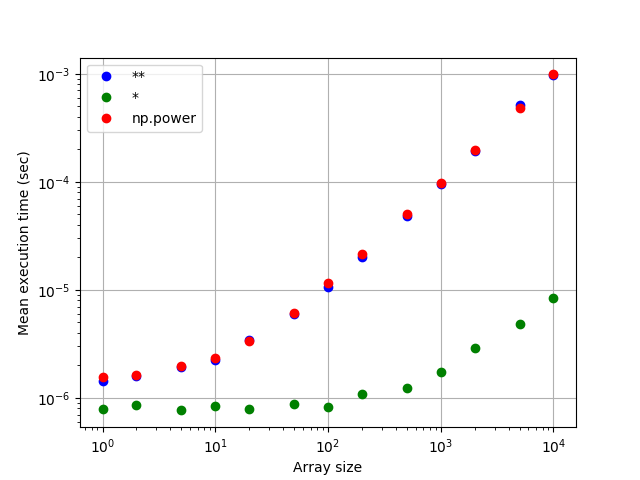
\includegraphics[width=0.97\linewidth]{figures/benchmark.png}
\caption{Approximate calculation time of the numpy \texttt{power} function, \texttt{**} operation, and the \texttt{*} operation on arrays of random positive floating point values.}\label{fig:benchmark}
\end{figure}

Because of the dominance of numerical overhead, repeated multiplication operations can be more expensive than a call to \texttt{power} on small arrays.  However, it should be emphasized that judicious use of computational effort is really only critical on large arrays, anyway.  For arrays with 100 elements, \texttt{power} operations are about 10 times as expensive, but \texttt{power} function calls on 10,000-element arrays are roughly equivalent to 100 multiplications.

This leads to a careful choice for arrays with large exponents (or tiny fractional values).  The large exponents in the last example can be mitigated at the cost of added overhead and complexity by splitting the polynomial into two separate polynomials, each with its own scaling.
\begin{align}
p(x,y) &= 2x^{-2} + x^{0.1}y + xy^2.\nonumber\\
 &= x^{-2} \left(2 + x^3y^2 \right) + x^{0.1} y\nonumber\\
\end{align}

\subsection{Representation of polynomials in data}

The \texttt{json} data representation of a polynomial on two dimensions uses three-deep series of nested lists to describe the pre- and post-exponents, the coefficients, and their corresponding exponents for multiple polynomial parts.  For example, the nested lists below define a polynomial with multiple parts.

\begin{lstlisting}{language=Python}
poly = [# This begins the list of sub-polynomials
    [# This begins the first sub-polynomial
        [<a>,<b>], 
        [<alpha>, <beta>],
        [<i0>, <j0>, <c0>],
        [<i1>, <j1>, <c1>],
        <...>
    ],
    [# This begins the second sub-polynomial
        [<a>,<b>], 
        [<alpha>, <beta>],
        [<i0>, <j0>, <c0>],
        [<i1>, <j1>, <c1>],
        <...>
    ],
    <...more sub-polynomials...>
]
\end{lstlisting}

The exponents \texttt{i0}, \texttt{j0}, \texttt{i1}, etc., must be non-negative integers listed in descending order, sorted by $i$ first and then sorted by $j$.  An alternative approach is to define a two-dimensional polynomial with a matrix of coefficients, each row and column corresponding to a power of $x$ or $y$, but that method suffers when there are only a few terms with high powers.  This approach might be called a ``sparse coordinate matrix'' approach to defining a polynomial.

\subsection{Efficient evaluation of the polynomial}

Once a polynomial is adjusted to use only non-negative integer exponents.
\begin{align}
p(x,y) = \sum_{i,j} c_{i,j} x^i y^j
\end{align}
However, evaluating each term individually requires two expensive calls to a \verb|pow| function and two floating point multiplications.

The widely accepted method for evaluating a polynomial of one variable is to construct a recursive expansion
\begin{align}
q(y) = c_0 + y ( c_1 + y ( c_2 + y ( \ldots
\end{align}
If there are $n$ coefficients, then this amounts to only $n$ multiplications with no \verb|pow| calls.  In order to extend this algorithm to two variables, more elegant notation will be helpful.  If we name the intermediate value calculated in the process of these recursions $q_j$, then a polynomial with $n$ terms implies the series
\begin{align}
q_n &= c_n\\
q_j(y) &= c_j + y\,q_{j+1}(y)\\
q_0(y) &= q(y).
\end{align}
This is a series beginning with $j=n$ and proceeding backwards to $j=0$.  The final function in the series, $q_0$ is also the desired polynomial, $q(y)$.  In practice, there is no need to keep the old values of $q$, so a single register may be used to hold the latest value.

How can this be extended to a polynomial of two variables?  We may consider the polynomials to be nested; the evaluation of a polynomial on $y$ determines the individual coefficients for a polynomial on $x$.
\begin{align}
p(x,y) &= \sum_i q_i(y) x^i\\
q_i(y) &= \sum_j c_{i,j} y^j
\end{align}

We only need a minor modification to the intermediate values for the $x$ polynomial since there will be a separate expansion for each value of $i$.  If there are $n$ $j$ terms,
\begin{subequations}
\begin{align}
q_{i,n}(y) &= c_{n,j}\\
q_{i,j}(y) &= c_{i,j} + y\,q_{i+1,j}(y)\\
q_{i,0}(y) &= q_i(y).
\end{align}
\end{subequations}

If there are $m$ $x$-terms,
\begin{subequations}
\begin{align}
p_m(x,y) &= q_m(y)\\
p_i(x,y) &= q_i(x) + y\,p_{i+1}(x,y)\\
p_0(x,y) &= p(x,y).
\end{align}
\end{subequations}

\subsection{Efficient evaluation of derivatives}

The partial derivatives of the polynomial can be efficiently evaluated along with the polynomial itself. To relax the already cumbersome notation, the functional dependencies $(y)$ and $(x,y)$ will be dropped.  For the purpose of thermodynamic property evaluation, the first two derivatives will suffice.

Let us begin with the simpler task of calculating the derivatives of $q_i$ with respect to $y$.
\begin{subequations}
\begin{align}
q_{i,n|y} &= 0\\
q_{i,j|y} &= q_{i+1,j} + y\,q_{i+1,j|y}\\
q_{i,0|y} &= q_{i|y}
\end{align}
\end{subequations}

\begin{subequations}
\begin{align}
q_{i,n|yy} &= 0\\
q_{i,j|yy} &= 2 q_{i,j+1|y} + y\,q_{i,j+1|yy}\\
q_{i,0|yy} &= q_{i|yy}
\end{align}
\end{subequations}

The derivatives on $p$ are constructed somewhat differently because they can be in both $x$ and $y$.  Beginning with $y$,
\begin{subequations}
\begin{align}
p_{n|y} &= 0\\
p_{j|y} &= q_{i|y} + x\,p_{j+1|y}\\
p_{0|y} &= p_y
\end{align}
\end{subequations}

\begin{subequations}
\begin{align}
p_{m|yy} &= 0\\
p_{i|yy} &= q_{i|yy} + x\,q_{i+1|yy}\\
p_{0|yy} &= p_{yy}
\end{align}
\end{subequations}

The derivatives on $x$ appear
\begin{subequations}
\begin{align}
p_{m|x} &= 0\\
p_{i|x} &= p_{i+1} + x\,p_{i+1|x}\\
p_{0|x} &= p_x
\end{align}
\end{subequations}

\begin{subequations}
\begin{align}
p_{n|xx} &= 0\\
p_{i|xx} &= 2 p_{i+1|x} + x\,p_{i+1|xx}\\
p_{0|xx} &= p_{xx}
\end{align}
\end{subequations}

Finally, the cross-term (both $x$ and $y$) appears
\begin{subequations}
\begin{align}
p_{n|xy} &= 0\\
p_{i|xy} &= p_{i+1|y} + y\,p_{i+1|xy}\\
p_{0|xy} &= p_{xy}
\end{align}
\end{subequations}

\subsection{Implementation of the algorithm}
In practice, this cumbersome notation can be drastically simplified in code because it is not necessary to distinguish between the subscripts of $p$ and $q$, provided care is taken not to overwrite a value before it is needed.

In most practical polynomials of two variables of order $m$ on $x$ and order $n$ on $y$, there are $(m+1)(n+1)$ possible coefficients, but many (if not most) of them may be zero.  As a result, storing the coefficient array in a 2D array (or matrix) format is not efficient.  Instead, \PM\ takes an approach closer to coordinate sparse matrix storage.

If we have one-dimensional arrays of polynomial coefficients, $c_k$, and exponents, $i_k$ and $j_k$, the polynomial will be constructed as
\begin{align}
p(X,Y) = \sum_k^{N-1} c_k X^{i_k} Y^{i_k}.
\end{align}
In this way, the polynomial
\begin{align}
p(X,Y) = -0.1 X^2 + XY + 0.5 Y^2 - Y - 0.2
\end{align}
may be represented by
\begin{align}
i &= \left[ 2,\ 1,\ 0,\ 0,\ 0\right]\\
j &= \left[ 0,\ 1,\ 2,\ 1,\ 0\right]\\
c &= \left[ -0.1,\ 1,\ 0.5,\ -1,\ 0.2\right]
\end{align}

For the algorithm to function efficiently, it is reasonable to impose some prior sorting of the exponent values.  Since the series developed in the previous section requires that we interact with higher-order terms first, let us assert that the polynomial should be expressed in order of descending exponents on $X$ and then $Y$.

In Algorithm \ref{alg:poly2}, an outer loop over the range of values of $i$ and an inner loop on the range of values of $j$ considers all of the possible terms in the polynomial.  If coefficients are absent from the arrays (if the $i,j$ pair is not found), then the term is not included in the polynomial (the coefficient is zero).  Starting with the maximum value for each exponent, the indices are reduced incrementally until the $i,j$ combination corresponding to the next row ($k$) is found.

\begin{algorithm}
\caption{Efficient evaluation of a polynomial of two variables}\label{alg:poly2}
\begin{algorithmic}[1]
\Procedure{\_poly2}{$x,y,i,j,c$} \Comment{$i,j,c$ are arrays}
\State $p, p_x, p_y, p_{xx}, p_{xy}, p_{yy} \gets 0$  \Comment{Initialize the results with zero}
\State $i_{max} \gets i[0]$  \Comment{Detect the maximum $i$ value}
\State $k \gets 0$ \Comment{$k$ is our place in the coefficient array}
\For{$ii=i_{max}$ to $0$}   \Comment{All possible $i$ values}
    \If{$k < N$ and $i[k]==ii$} \Comment{Is there an $x^{ii}$ term?}
        \State $j_{max} \gets j[k]$ \Comment{Detect the maximum $j$ value}
        \State $q,q_y,q_{yy} \gets 0$   \Comment{Initialize the inner $q$ result}
        \For{$jj=j_{max}$ to $0$} \Comment{All possible $j$ values}
            \State $q_{yy} \gets 2 q_y + y q_{yy}$
            \State $q_y \gets q + y q_y$
            \If{$k<N$ and $a_k$ is $i$ and $b_k$ is $j$}  \Comment{Is there a $x^{ii}y^{jj}$ term?}
                \State $q \gets c_k + y q$
                \State $k \gets k+1$
            \Else   \Comment{Term not in polynomial}
                \State $q \gets y q$
            \EndIf
        \EndFor
        \State $p_{yy} \gets q_{yy} + x p_{yy}$
        \State $p_{xx} \gets 2 p_x + x p_{xx}$
        \State $p_{xy} \gets p_y + x p_{xy}$
        \State $p_x \gets p + x p_x$
        \State $p_y \gets q_y + x p_y$
        \State $p \gets q + x p$
    \Else \Comment{Term not in polynomial}
        \State $p_{yy} \gets x p_{yy}$
        \State $p_{xx} \gets 2 p_x + x p_{xx}$
        \State $p_{xy} \gets p_y + x p_{xy}$
        \State $p_x \gets p + x p_x$
        \State $p_y \gets x p_y$
        \State $p \gets x p$
    \EndIf
\EndFor
\State \Return $p,p_x,p_y,p_{xx},p_{xy},p_{yy}$
\EndProcedure
\end{algorithmic}
\end{algorithm}

\section{Polynomials in one dimension}\label{sec:num:poly1}

Polynomials of one dimension benefit from the same approach as two-dimensional polynomials, but the algorithm is far simpler.  All the formulae and algorithms that apply to $q$ in the last section may simply be repurposed for a single dimensional polynomial.  

The only topic that really requires special treatment is the format used in data.  One-dimensional polynomials are identical to two-dimensional polynomials, except (1) the pre- and post-exponent values are scalars instead of two-element lists, and (2) each term only needs two parameters instead of three.

\begin{lstlisting}[language=Python]
coef = [ # begins the polynomial
    [ # begins a sub-polynomial
        <a>, 
        <alpha>,
        [ <i0>, <c0> ],
        [ <i1>, <c1> ],
        <...>
    ],
    [ # begins a second sub-polynomial
        <a>, 
        <alpha>,
        [ <i0>, <c0> ],
        [ <i1>, <c1> ],
        <...>
    ],
    <... more sub-polynomials?...>
]
\end{lstlisting}

\section{Iteration with \texttt{iter1}}\label{sec:num:iter1}

Most of the classes have a member that implements some variation of the Newton-Rhapson variant \verb|_iter1| method.  It is fast, and it has excellent convergence characteristics in most applications except the numerically irksome cases found in the multi-phase models.

Given a function on one variable, $f$, the \verb|_iter1| algorithm seeks a value, $x$, between upper and lower limits, $x_{max}$ and $x_{min}$ so that $f(x)$ is equal to a reference value, $y$.  

Given a guess, $x_k$, traditional Newton-Rhapson iteration calculates a next guess, $x_{k+1}$ by extrapolating linearly,
\begin{align}
\Delta x &= \frac{y-f(x_k)}{f'(x_k)}\\
x_{k+1} &= x_k + \Delta x.
\end{align}
This is simply repeated until $y-f(x_k)$ is sufficiently small.

However, in problems with substantial nonlinearities, the iteration can diverge badly like in Figure \ref{fig:iter1}.  Worse still, these intermediate guesses can even wander to illegal property values.

\begin{figure}
\centering
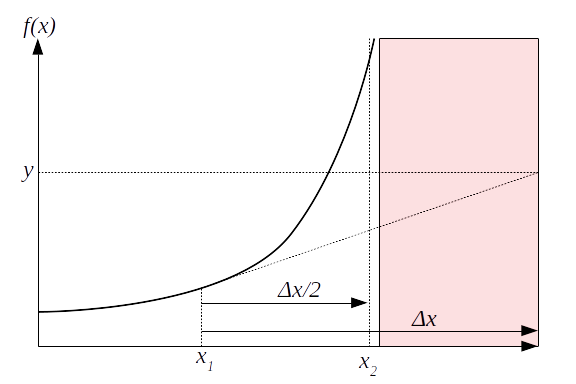
\includegraphics[width=0.97\linewidth]{figures/iter1}
\caption{An example of a system where classical Newton iteration diverges to illegal values.  The }\label{fig:iter1}
\end{figure}

The \verb|_iter1| algorithm addresses the problem by allowing the calling property method to establish upper and lower boundaries on the value, $x$.  If a guess wanders outside of the valid range, the size of the step, $\Delta x$, is halved repeatedly until the next guess is back in the valid range.  The algorithm is usually initialized externally with some first guess for $x$.

\begin{algorithm}
\caption{ITER1: Modified bounded Newton-Rhapson iteration, $y = f(x)$}\label{alg:iter1}
\begin{algorithmic}
\Procedure{\_iter1}{$f,y,x_{min},x_{max},x,\epsilon$}
\State $x_k \gets x$ \Comment{Initialize the current guess}
\State $y_k \gets f(x)$ \Comment{Evaluate the function}
\State $y'_k \gets f'(x)$
\While{$|y-y_k| > \epsilon$} \Comment{While error is large}
\State $\Delta x \gets (y - y_k)/y'_k$ \Comment{Calculate step size}
\State $x_{k+1} \gets x_k + \Delta x$ \Comment{Calculate the next guess}
\State \Comment{If $x_k$ is out of bounds}
\While{$x_{k+1} > x_{max}$ or $x_{k+1} < x_{min}$} 
\State $\Delta x \gets \Delta x / 2$ \Comment{Halve $\Delta x$}
\State $x_{k+1} \gets x_k + \Delta x$ \Comment{Update the guess}
\EndWhile
\State $x_{k} \gets x_{k+1}$ \Comment{Accept the new guess}
\State $y_k \gets f(x_k)$ \Comment{Evaluate the function}
\State $y'_k \gets f'(x_k)$
\EndWhile
\State \Return $x_k$
\EndProcedure
\end{algorithmic}
\end{algorithm}

Algorithm \ref{alg:iter1} gives a simplified version of the algorithm implemented in \PM.  See the in-line documentation and comments for a more detailed description.

\section{Iteration with \texttt{hybrid1}}\label{sec:num:hybrid1}

Multi-phase properties present severe numerical challenges since the phase change represents an abrupt jump in properties, and the iteration is inherently two-dimensional.  The \verb|_iter1| algorithm prevents the solution from diverging, but it often fails to converge in multi-phase substance inversion problems.

\subsection{Bisection iteration}\label{sec:num:bisection}

Bisection is a classic approach to nasty inversion problems where Newton iteration fails.  If upper and lower bounds, $x_a$ and $x_b$ are found so that $f(x_a) < y < f(x_b)$, then a continuous function must have a value somewhere between $x_a$ and $x_b$ such that $f(x) = y$.  If we were to divide the domain in half $x_c = (x_a+x_b)/2$ and evaluate the function there, its value will either be above or below $y$, so one of the two values could be replaced by $x_c$.  In this way, the domain between $x_a$ and $x_b$ is reliably cut in half with every iteration step, no matter how bizarrely $f(x)$ behaves.

This process just has to be repeated until the distance between the upper and lower bounds have shrunk to be so small that the numerical uncertainty is acceptable.  Figure \ref{fig:bisection} shows three steps using this process.  The vertical space occupied by each blue box represents the shrinking uncertainty for the value of $f(x)$ and the horizontal space represents the shrinking uncertainty in $x$.

\begin{figure}
\centering
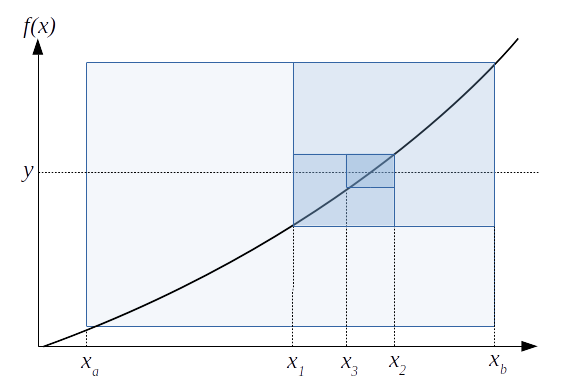
\includegraphics[width=0.97\linewidth]{figures/bisection}
\caption{A depiction of the bisection iteration algorithm on a hypothetical function.}\label{fig:bisection}
\end{figure}

While Newton iteration might converge in only a few steps on a nearly linear function, bisection can take tens of steps depending on the ratio of the initial domain and the acceptable error range.  Since the domain is divided by two every time, it is easy to calculate the number of iterations to obtain a certain domain size.
\begin{align}
N = \log_2 \frac{|x_b - x_a|}{\epsilon}
\end{align}
If the initial domain were a temperature range of 0 to 1000 Kelvin, and the acceptable error were .01 Kelvin, 17 iterations are required.  If the acceptable error were tightened to .001 Kelvin, 20 iterations are required!

\subsection{The \texttt{hybrid1} candidates}

Literature on numerical methods is littered with different flavors of hybrid algorithms that try to benefit from the guaranteed convergence of bisection and the speed of Newton-Rhapson.  This algorithm is specifically designed for application on the types of functions that appear in thermodynamic properties.

This hybrid approach begins by bracketing a solution with guesses, $x_a$ and $x_b$, just like a bisection algorithm.  Then, we calculate three candidates for the next guess, $x_c$:

1. Newton iteration from $x_a$: 
\begin{align}
x_1 = x_a + \frac{y-f(x_a)}{f'(x_a)}
\end{align}

2. Newton iteration from $x_b$:
\begin{align}
x_2 = x_b + \frac{y-f(x_b)}{f'(x_b)}
\end{align}

3. Bisection iteration from $x_a$ and $x_b$:
\begin{align}
x_3 = \frac{x_a + x_b}{2}
\end{align}

These three parallel processes for calculating candidates are shown in Figure \ref{fig:hybrid}.  As the next sections will explore, the next step is to select one.  Once the function is evaluated there, the boundaries can be updated (just like in bisection) and convergence can be tested.

\begin{figure}
\centering
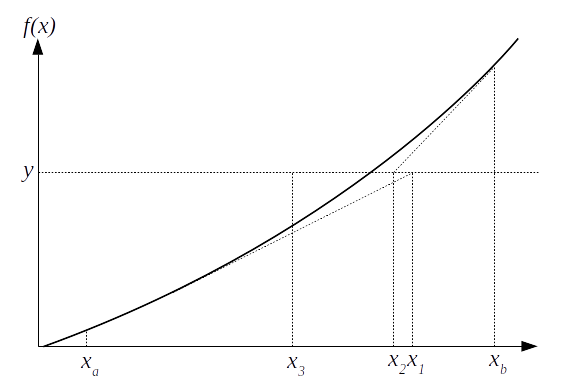
\includegraphics[width=0.97\linewidth]{figures/hybrid1}
\caption{A depiction of the bisection iteration algorithm on a hypothetical function.}\label{fig:hybrid}
\end{figure}

One could pose dozens of ideas for how information about these three candidates might be used to select a best guess, but only two are implemented in \PM.  They are discussed in the sections below.

It may appear that each iteration requires two function evaluations, but that is not so.  The next guess will be used to replace either the upper or lower bound (and its candidate).  The function values and the candidate for the other bound can be retained.

\subsection{Standard candidate selection}

Once the candidate guesses are calculated, the next step is to select a single candidate for the next step of iteration.  In general, the Newton steps at the extremes of the domain are unlikely to be very good until the algorithm is very close to the solution.  If the two Newton iteration steps produce a guess very close to each other, there is a good chance that they can be trusted.  Otherwise, it is probably best to rely on the bisection step.  Above all, it is vital that no guess ever lie outside of the boundaries where a solution is known to exist.

In standard candidate selection, the median (middle) of the three guesses is selected.  If the median lies outside of $x_a$ and $x_b$, then the next guess reverts to the bisection.  In this way, if the two guesses at the edge agree, the more conservative of the two (the one closer to the center of the domain) will be selected.  If they disagree or if they both diverge from the domain, the algorithm reverts to bisection.

\begin{algorithm}
\caption{HYBRID1: Hybrid bisection and Newton iteration}\label{alg:hybrid1}
\begin{algorithmic}
\Procedure{\_hybrid1}{$f,y,x_a,x_b,\epsilon_x,\epsilon_y$}
\State $y_a \gets f(x_a)$   \Comment{Evaluate $f$ at the initial bounds}
\State $y'_a \gets f'(x_a)$
\State $y_b \gets f(x_b)$
\State $y'_b \gets f'(x_b)$
\If{$y_a > y_b$}
    \State $x_a,y_a,y'_a \leftrightarrow x_b,y_b,y'_b$  \Comment{Swap the bounds}
\EndIf
\If{NOT $y_a < y < y_b$}
    \State \Return ``ERROR: The solution is not bracketed''
\EndIf
\State $x_1 \gets x_a + (y-y_a)/y'_a$   \Comment{The first candidates}
\State $x_2 \gets x_b + (y-y_b)/y'_b$
\State $x_3 \gets (x_a + x_b)/2$
\While{$|x_b-x_a|> \epsilon_x$}     \Comment{Halt if the interval is small}
    \State $x_c \gets \mathrm{median}(x_1,x_2,x_3)$ \Comment{Select the median}
    \If{$x_c \le \mathrm{min}(x_a,x_b)$ OR $x_c \ge \mathrm{max}(x_a,x_b)$} \Comment{If out of bounds...}
        \State $x_c \gets x_3$ \Comment{...use bisection instead}
    \EndIf
    \State $y_c \gets f(x_c)$ \Comment{Evaluate $f$ at the new guess}
    \State $y'_c\gets f'(x_c)$ 
    \If{$|y_c - y| < \epsilon_y$} \Comment{Test for Newton convergence}
        \State \Return $x_c$
    \EndIf
    \If{$y_c < y$} \Comment{If this is a lower bound}
        \State $x_a \gets x_c$ \Comment{Replace the lower bound}
        \State $y_a \gets y_c$
        \State $y'_a \gets y'_c$
        \State $x_1 \gets x_a + (y - y_a)/y'_a$ \Comment{A new lower candidate}
        \State \ldots
\algstore{algs:hybrid1}
\end{algorithmic}
\end{algorithm}

\begin{algorithm}
\caption{HYBRID1: Hybrid bisection continued}
\begin{algorithmic}
\algrestore{algs:hybrid1}
        \State \ldots
    \Else \Comment{If this is an upper bound}
        \State $x_b \gets x_c$ \Comment{Replace the upper bound}
        \State $y_b \gets y_c$
        \State $y'_b \gets y'_c$
        \State $x_2 \gets x_b + (y - y_b)/y'_b$ \Comment{A new upper candidate}
    \EndIf
    \State $x_3 = (x_a + x_b)/2$    \Comment{A new bisection candidate}
\EndWhile
\State \Return $x_3$    \Comment{Convergence by bisection}
\EndProcedure
\end{algorithmic}
\end{algorithm}

The standard candidate selection process gives excellent performance virtually everywhere in multi-phase property domains except very near the critical point.  Testing revealed that standard candidate selection is vulnerable to slow convergence near the critical point due to the extreme numerical stiffness there.  It should be emphasized that the algorithm still converges; just very slowly.

The problem is similar to one that happens in the secant iteration algorithm.  If a solution lies in a numerically stiff regime like in Figure \ref{fig:bisection}, the boundary at the stiff edge will produce a guess very close to itself while the other guess will produce a guess that diverges outside the boundary.  Median candidate selection will always favor the candidate at the stiff edge even though it only barely moves from the one prior.

\subsection{Paranoid candidate selection}

So-called ``paranoid'' candidate selection utterly distrusts the Newton method if either of the guesses lie outside of the domain.  The idea is that if the domain is so nonlinear that either of the guesses leaves the domain, the algorithm should revert to bisection until it looks like the function is locally linear.

\begin{algorithm}
\caption{HYBRID1: Paranoid hybrid iteration}\label{alg:hybrid1:paranoid}
\begin{algorithmic}
\Procedure{\_hybrid1}{$f,y,x_a,x_b,\epsilon_x, \epsilon_y$}
\State $y_a \gets f(x_a)$   \Comment{Evaluate $f$ at the initial bounds}
\State $y'_a \gets f'(x_a)$
\State $y_b \gets f(x_b)$
\State $y'_b \gets f'(x_b)$
\If{$y_a > y_b$}
    \State $x_a,y_a,y'_a \leftrightarrow x_b,y_b,y'_b$  \Comment{Swap the bounds}
\EndIf
\If{NOT $y_a < y < y_b$}
    \State \Return ``ERROR: The solution is not bracketed''
\EndIf
\State $x_1 \gets x_a + (y-y_a)/y'_a$   \Comment{The first candidates}
\State $x_2 \gets x_b + (y-y_b)/y'_b$
\State $x_3 \gets (x_a + x_b)/2$
\While{$|x_b-x_a|> \epsilon_x$}     \Comment{Halt if the interval is small}
    \State \Comment{If either guess is out of bounds...}
    \If{$x_1 \notin (x_a,x_b)$ OR $x_2 \notin (x_a,x_b)$} 
        \State $x_c \gets x_3$ \Comment{...use bisection instead}
    \Else
        \State $x_c \gets \mathrm{median}(x_1,x_2,x_3)$ \Comment{Select the median}
    \EndIf
    \State $y_c \gets f(x_c)$ \Comment{Evaluate $f$ at the new guess}
    \State $y'_c\gets f'(x_c)$ 
    \If{$|y_c - y| < \epsilon_y$} \Comment{Test for Newton convergence}
        \State \Return $x_c$
    \EndIf
    \If{$y_c < y$} \Comment{If this is a lower bound}
        \State $x_a \gets x_c$ \Comment{Replace the lower bound}
        \State $y_a \gets y_c$
        \State $y'_a \gets y'_c$
        \State $x_1 \gets x_a + (y - y_a)/y'_a$ \Comment{A new lower candidate}
        \State \ldots
\algstore{algs:hybrid1:paranoid}
\end{algorithmic}
\end{algorithm}

\begin{algorithm}
\caption{HYBRID1: Paranoid hybrid iteration continued}
\begin{algorithmic}
\algrestore{algs:hybrid1:paranoid}
        \State \ldots
    \Else \Comment{If this is an upper bound}
        \State $x_b \gets x_c$ \Comment{Replace the upper bound}
        \State $y_b \gets y_c$
        \State $y'_b \gets y'_c$
        \State $x_2 \gets x_b + (y - y_b)/y'_b$ \Comment{A new upper candidate}
    \EndIf
    \State $x_3 = (x_a + x_b)/2$    \Comment{A new bisection candidate}
\EndWhile
\State \Return $x_3$    \Comment{Convergence by bisection}
\EndProcedure
\end{algorithmic}
\end{algorithm}

In practice, paranoid hybrid iteration is slower than standard hybrid iteration.  However, in testing, it has never failed to converge on any of the multi-phase models.  Under the most difficult conditions, it might take ten or more iterations to converge.  In better conditions, it typically converges in five or so iterations.
